\documentclass{article}\usepackage[]{graphicx}\usepackage[]{color}
%% maxwidth is the original width if it is less than linewidth
%% otherwise use linewidth (to make sure the graphics do not exceed the margin)
\makeatletter
\def\maxwidth{ %
  \ifdim\Gin@nat@width>\linewidth
    \linewidth
  \else
    \Gin@nat@width
  \fi
}
\makeatother

\definecolor{fgcolor}{rgb}{0.345, 0.345, 0.345}
\newcommand{\hlnum}[1]{\textcolor[rgb]{0.686,0.059,0.569}{#1}}%
\newcommand{\hlstr}[1]{\textcolor[rgb]{0.192,0.494,0.8}{#1}}%
\newcommand{\hlcom}[1]{\textcolor[rgb]{0.678,0.584,0.686}{\textit{#1}}}%
\newcommand{\hlopt}[1]{\textcolor[rgb]{0,0,0}{#1}}%
\newcommand{\hlstd}[1]{\textcolor[rgb]{0.345,0.345,0.345}{#1}}%
\newcommand{\hlkwa}[1]{\textcolor[rgb]{0.161,0.373,0.58}{\textbf{#1}}}%
\newcommand{\hlkwb}[1]{\textcolor[rgb]{0.69,0.353,0.396}{#1}}%
\newcommand{\hlkwc}[1]{\textcolor[rgb]{0.333,0.667,0.333}{#1}}%
\newcommand{\hlkwd}[1]{\textcolor[rgb]{0.737,0.353,0.396}{\textbf{#1}}}%

\usepackage{framed}
\makeatletter
\newenvironment{kframe}{%
 \def\at@end@of@kframe{}%
 \ifinner\ifhmode%
  \def\at@end@of@kframe{\end{minipage}}%
  \begin{minipage}{\columnwidth}%
 \fi\fi%
 \def\FrameCommand##1{\hskip\@totalleftmargin \hskip-\fboxsep
 \colorbox{shadecolor}{##1}\hskip-\fboxsep
     % There is no \\@totalrightmargin, so:
     \hskip-\linewidth \hskip-\@totalleftmargin \hskip\columnwidth}%
 \MakeFramed {\advance\hsize-\width
   \@totalleftmargin\z@ \linewidth\hsize
   \@setminipage}}%
 {\par\unskip\endMakeFramed%
 \at@end@of@kframe}
\makeatother

\definecolor{shadecolor}{rgb}{.97, .97, .97}
\definecolor{messagecolor}{rgb}{0, 0, 0}
\definecolor{warningcolor}{rgb}{1, 0, 1}
\definecolor{errorcolor}{rgb}{1, 0, 0}
\newenvironment{knitrout}{}{} % an empty environment to be redefined in TeX

\usepackage{alltt}
\IfFileExists{upquote.sty}{\usepackage{upquote}}{}
\begin{document}

\begin{knitrout}
\definecolor{shadecolor}{rgb}{0.969, 0.969, 0.969}\color{fgcolor}\begin{kframe}
\begin{alltt}
\hlcom{#GUIA 15}

\hlstd{x} \hlkwb{<-} \hlnum{55}\hlstd{; a}\hlkwb{=}\hlnum{0}\hlstd{; b} \hlkwb{<-} \hlnum{90}
\hlcom{#usando la funci�n propia de R}
\hlkwd{punif}\hlstd{(x,} \hlkwc{min}\hlstd{=a,} \hlkwc{max}\hlstd{=b,} \hlkwc{lower.tail}\hlstd{=}\hlnum{TRUE}\hlstd{)}
\end{alltt}
\begin{verbatim}
## [1] 0.6111111
\end{verbatim}
\begin{alltt}
\hlstd{F55}\hlkwb{=}\hlkwd{punif}\hlstd{(}\hlnum{55}\hlstd{,} \hlkwc{min}\hlstd{=a,} \hlkwc{max}\hlstd{=b,} \hlkwc{lower.tail}\hlstd{=}\hlnum{TRUE}\hlstd{)}
\hlstd{F15}\hlkwb{=}\hlkwd{punif}\hlstd{(}\hlnum{15}\hlstd{,} \hlkwc{min}\hlstd{=a,} \hlkwc{max}\hlstd{=b,} \hlkwc{lower.tail}\hlstd{=}\hlnum{TRUE}\hlstd{)}
\hlstd{F55}\hlopt{-}\hlstd{F15}
\end{alltt}
\begin{verbatim}
## [1] 0.4444444
\end{verbatim}
\begin{alltt}
\hlstd{F55}\hlkwb{=}\hlkwd{punif}\hlstd{(}\hlnum{55}\hlstd{,} \hlkwc{min}\hlstd{=a,} \hlkwc{max}\hlstd{=b,} \hlkwc{lower.tail}\hlstd{=}\hlnum{TRUE}\hlstd{);F55}
\end{alltt}
\begin{verbatim}
## [1] 0.6111111
\end{verbatim}
\begin{alltt}
\hlcom{#Luego multiplicando ambas probabilidades se obtiene el valor pedido 0.1728.}
\hlstd{(}\hlnum{1}\hlopt{-}\hlstd{F55)}\hlopt{*}\hlstd{( F55}\hlopt{-}\hlstd{F15)}
\end{alltt}
\begin{verbatim}
## [1] 0.1728395
\end{verbatim}
\begin{alltt}
\hlcom{#y los cuantiles-normales para la variable X:}
\hlstd{p} \hlkwb{<-} \hlkwd{c}\hlstd{(}\hlnum{0.80}\hlstd{); media}\hlkwb{=}\hlnum{5}\hlstd{; d.t}\hlkwb{=}\hlnum{1}
\hlkwd{qnorm}\hlstd{(p,} \hlkwc{mean}\hlstd{=media,} \hlkwc{sd}\hlstd{=d.t,} \hlkwc{lower.tail}\hlstd{=}\hlnum{TRUE}\hlstd{)}
\end{alltt}
\begin{verbatim}
## [1] 5.841621
\end{verbatim}
\begin{alltt}
\hlcom{#y los cuantiles-t para la variable Y:}
\hlstd{p} \hlkwb{<-} \hlkwd{c}\hlstd{(}\hlnum{0.80}\hlstd{); g.l} \hlkwb{<-} \hlnum{10}
\hlkwd{qt}\hlstd{(p,} \hlkwc{df}\hlstd{=g.l,} \hlkwc{lower.tail}\hlstd{=}\hlnum{TRUE}\hlstd{)}
\end{alltt}
\begin{verbatim}
## [1] 0.8790578
\end{verbatim}
\begin{alltt}
\hlcom{#Como se desea calcular P(x ??? 4.5) :}
\hlstd{n} \hlkwb{<-} \hlnum{16}\hlstd{; x} \hlkwb{<-} \hlnum{4.5}\hlstd{; mu}\hlkwb{=}\hlnum{5}\hlstd{; sigma}\hlkwb{=}\hlnum{1}\hlstd{; d.t}\hlkwb{=}\hlstd{sigma}\hlopt{/}\hlkwd{sqrt}\hlstd{(n)}
\hlkwd{pnorm}\hlstd{(x,} \hlkwc{mean}\hlstd{=mu,} \hlkwc{sd}\hlstd{=d.t,} \hlkwc{lower.tail}\hlstd{=}\hlnum{FALSE}\hlstd{)}
\end{alltt}
\begin{verbatim}
## [1] 0.9772499
\end{verbatim}
\begin{alltt}
\hlcom{#La probabilidad P(X ??? 5) se obtiene as�:}
\hlstd{x} \hlkwb{<-} \hlnum{5}\hlstd{; teta}\hlkwb{=}\hlnum{7}
\hlkwd{pexp}\hlstd{(x,} \hlkwc{rate}\hlstd{=}\hlnum{1}\hlopt{/}\hlstd{teta,} \hlkwc{lower.tail}\hlstd{=}\hlnum{FALSE}\hlstd{)}
\end{alltt}
\begin{verbatim}
## [1] 0.4895417
\end{verbatim}
\begin{alltt}
\hlcom{#y de igual forma P(X < 3) :}
\hlstd{x} \hlkwb{<-} \hlnum{3}\hlstd{; teta}\hlkwb{=}\hlnum{7}
\hlkwd{pexp}\hlstd{(x,} \hlkwc{rate}\hlstd{=}\hlnum{1}\hlopt{/}\hlstd{teta,} \hlkwc{lower.tail}\hlstd{=}\hlnum{TRUE}\hlstd{)}
\end{alltt}
\begin{verbatim}
## [1] 0.3485609
\end{verbatim}
\begin{alltt}
\hlkwd{pexp}\hlstd{(}\hlnum{4}\hlstd{,} \hlkwc{rate}\hlstd{=}\hlnum{1}\hlopt{/}\hlstd{teta,} \hlkwc{lower.tail}\hlstd{=}\hlnum{FALSE}\hlstd{)}
\end{alltt}
\begin{verbatim}
## [1] 0.5647181
\end{verbatim}
\begin{alltt}
\hlcom{#Hay que calcular el percentil 90:}
\hlstd{p} \hlkwb{<-} \hlnum{0.9}\hlstd{; teta} \hlkwb{<-} \hlnum{7}
\hlkwd{qexp}\hlstd{(p,} \hlkwc{rate}\hlstd{=}\hlnum{1}\hlopt{/}\hlstd{teta,} \hlkwc{lower.tail}\hlstd{=}\hlnum{TRUE}\hlstd{)}
\end{alltt}
\begin{verbatim}
## [1] 16.1181
\end{verbatim}
\begin{alltt}
\hlcom{#resultando 16.12 a�os.}

\hlkwd{qexp}\hlstd{(}\hlnum{0.5}\hlstd{,} \hlkwc{rate}\hlstd{=}\hlnum{1}\hlopt{/}\hlstd{teta,} \hlkwc{lower.tail}\hlstd{=}\hlnum{TRUE}\hlstd{)}
\end{alltt}
\begin{verbatim}
## [1] 4.85203
\end{verbatim}
\begin{alltt}
\hlcom{#y en el segundo caso, el percentil 68, b = 7.97}
\hlkwd{qexp}\hlstd{(}\hlnum{0.68}\hlstd{,} \hlkwc{rate}\hlstd{=}\hlnum{1}\hlopt{/}\hlstd{teta,} \hlkwc{lower.tail}\hlstd{=}\hlnum{TRUE}\hlstd{)}
\end{alltt}
\begin{verbatim}
## [1] 7.97604
\end{verbatim}
\begin{alltt}
\hlcom{#o de esta otra manera}
\hlkwd{qexp}\hlstd{(}\hlnum{0.32}\hlstd{,} \hlkwc{rate}\hlstd{=}\hlnum{1}\hlopt{/}\hlstd{teta,} \hlkwc{lower.tail}\hlstd{=}\hlnum{FALSE}\hlstd{)}
\end{alltt}
\begin{verbatim}
## [1] 7.97604
\end{verbatim}
\begin{alltt}
\hlcom{# Definir los par�metros apropiados}
\hlstd{min} \hlkwb{<-} \hlopt{-}\hlnum{2}\hlstd{; max} \hlkwb{<-} \hlnum{4}
\hlcom{# generar 100 n�meros aleatorios de la distribuci�n}
\hlstd{x} \hlkwb{=} \hlkwd{runif}\hlstd{(}\hlnum{100}\hlstd{, min, max); x}
\end{alltt}
\begin{verbatim}
##   [1] -1.78672151  0.85148167  1.12108331  2.94604945  1.85549998
##   [6] -0.10239208  2.74980291  2.80787862 -1.52833875  0.40530748
##  [11]  2.05157856  3.70321236 -1.60565074 -0.87015618  0.92881572
##  [16] -1.55256795 -0.61725472  3.04658179  0.82549123 -0.30499210
##  [21]  1.56175958  2.63558638 -1.54437910  1.59376547  0.33532904
##  [26]  2.04604289  1.43658819 -1.87119228  2.16550460  0.34940446
##  [31]  1.78040802 -0.75552233 -0.41103175 -0.66404002  0.20232600
##  [36] -0.59240274  2.60445342  3.57645639  3.71405089  2.94699732
##  [41] -0.18213900  1.01361124  2.93989904  3.33712766  1.74952192
##  [46]  3.34520821 -0.02171428  3.02379991 -1.34041660 -0.51851305
##  [51]  0.16958473  3.50735721 -0.95405323 -0.90590808  1.25112336
##  [56]  0.15536461  0.66958083 -0.32527305  1.93682252  1.01384368
##  [61]  3.92737085  1.54075329  0.52211769  3.28633773 -0.59121128
##  [66]  1.45632177  2.32490851  0.35540944  0.55875677  1.50443290
##  [71] -1.35523254 -1.86720029  0.10356513 -0.90074222 -1.17610321
##  [76]  1.88856098 -0.20652818  3.13401175 -0.60038070  0.23658700
##  [81]  3.18489457 -1.03450437 -0.18819307  2.42355529  2.15219891
##  [86]  2.01921593 -1.10257699 -1.17598028 -1.18196594  2.34052945
##  [91]  0.03049696 -1.87056786 -1.12698389  2.90228020  0.42798421
##  [96]  2.33321620  3.56270414 -1.70632363 -1.42930933  2.96808952
\end{verbatim}
\begin{alltt}
\hlcom{# Histograma para la nuestra aleatoria de tama�o 100}
\hlkwd{hist}\hlstd{(x,} \hlkwc{main}\hlstd{=}\hlstr{"X ~ Uniforme(min=-2, max=4"}\hlstd{,} \hlkwc{xlab}\hlstd{=}\hlstr{"X"}\hlstd{,} \hlkwc{ylab}\hlstd{=}\hlstr{"densidad de probabilidad"}\hlstd{,}
\hlkwc{probability}\hlstd{=}\hlnum{TRUE}\hlstd{,} \hlkwc{col}\hlstd{=}\hlstr{"green"}\hlstd{)}
\hlcom{# Graficar la funci�n de densidad, use la funci�n curve() para variable continua}
\hlkwd{curve}\hlstd{(}\hlkwd{dunif}\hlstd{(x, min, max),} \hlkwc{col}\hlstd{=}\hlstr{"blue"}\hlstd{,} \hlkwc{add}\hlstd{=}\hlnum{TRUE}\hlstd{)}
\end{alltt}
\end{kframe}
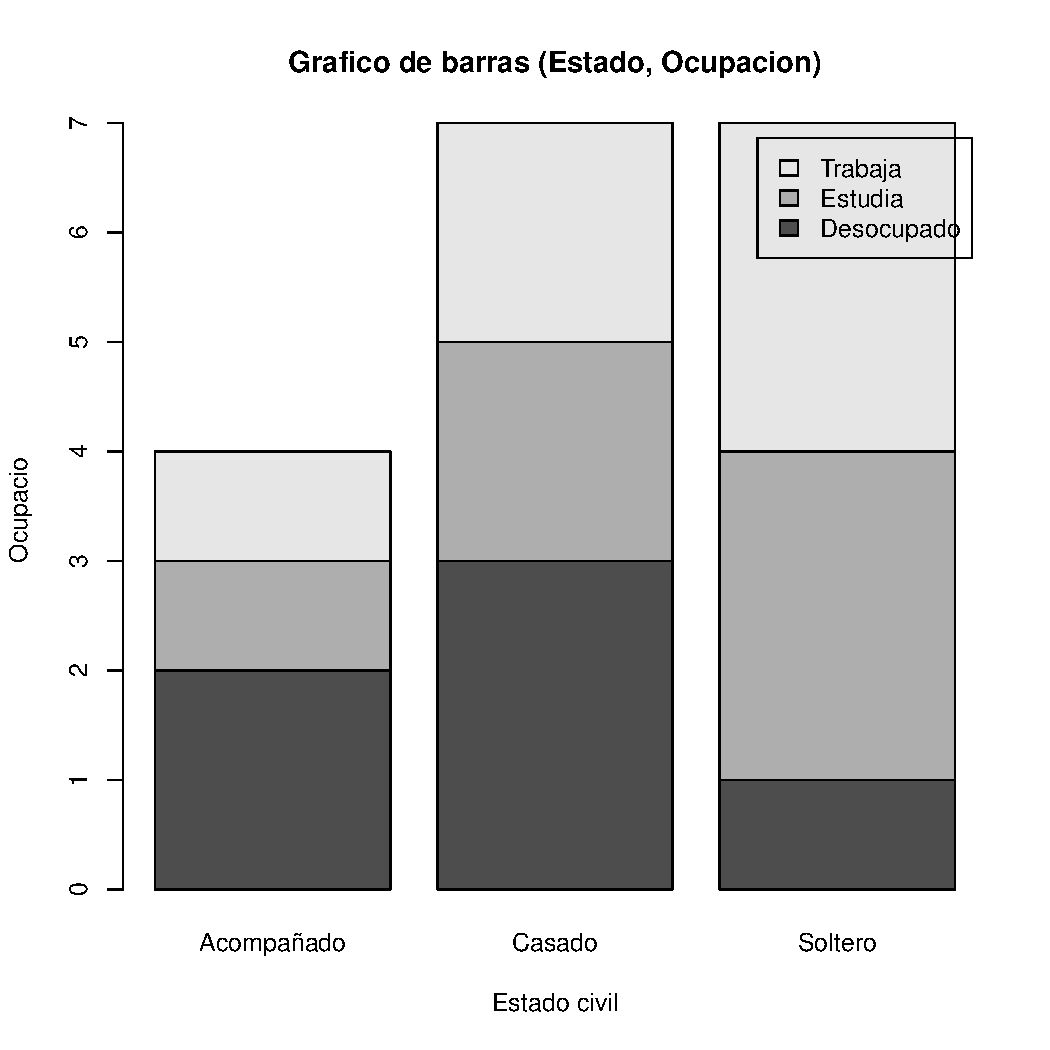
\includegraphics[width=\maxwidth]{figure/unnamed-chunk-1-1} 
\begin{kframe}\begin{alltt}
\hlcom{#genera los valores aleatorios de la distribuci�n}
\hlstd{x.norm} \hlkwb{<-} \hlkwd{rnorm}\hlstd{(}\hlkwc{n}\hlstd{=}\hlnum{200}\hlstd{,}\hlkwc{mean}\hlstd{=}\hlnum{10}\hlstd{,} \hlkwc{sd}\hlstd{=}\hlnum{2}\hlstd{)}

\hlcom{# Podemos obtener un histograma usando la funci�n hist()}
\hlkwd{hist}\hlstd{(x.norm,} \hlkwc{breaks} \hlstd{=} \hlstr{"Sturges"}\hlstd{,} \hlkwc{freq} \hlstd{=} \hlnum{TRUE}\hlstd{,} \hlkwc{probability} \hlstd{=} \hlnum{FALSE}\hlstd{,} \hlkwc{include.lowest} \hlstd{=} \hlnum{TRUE}\hlstd{,} \hlkwc{right}
\hlstd{=} \hlnum{TRUE}\hlstd{,} \hlkwc{density} \hlstd{=} \hlkwa{NULL}\hlstd{,} \hlkwc{angle} \hlstd{=} \hlnum{45}\hlstd{,} \hlkwc{col} \hlstd{=} \hlstr{"steelblue1"}\hlstd{,} \hlkwc{border} \hlstd{=} \hlkwa{NULL}\hlstd{,} \hlkwc{main} \hlstd{=} \hlstr{"Histograma de
datos observados"}\hlstd{,} \hlkwc{axes} \hlstd{=} \hlnum{TRUE}\hlstd{,} \hlkwc{plot} \hlstd{=} \hlnum{TRUE}\hlstd{,} \hlkwc{labels} \hlstd{=} \hlnum{FALSE}\hlstd{)}
\end{alltt}
\end{kframe}
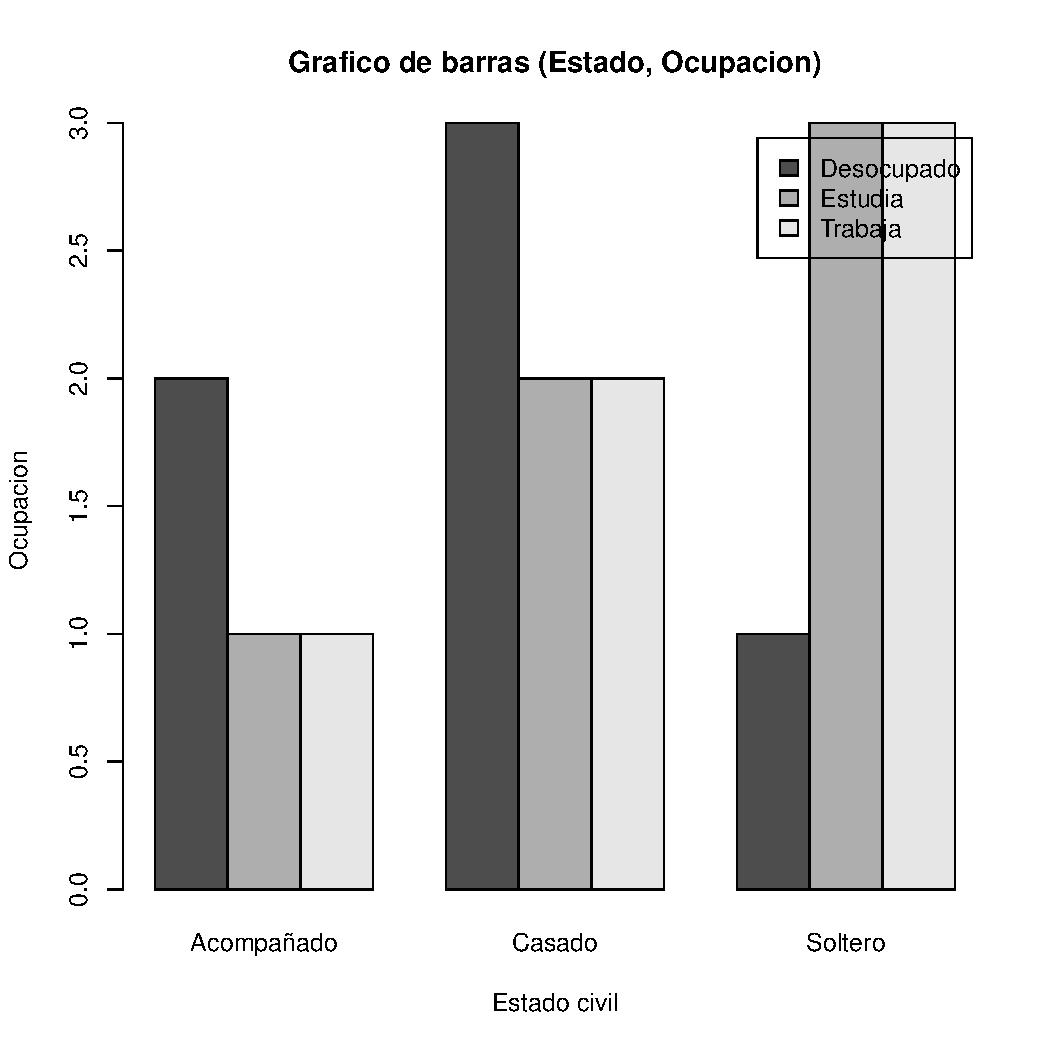
\includegraphics[width=\maxwidth]{figure/unnamed-chunk-1-2} 
\begin{kframe}\begin{alltt}
\hlkwd{plot}\hlstd{(}\hlkwd{density}\hlstd{(x.norm),} \hlkwc{main}\hlstd{=}\hlstr{"Densidad estimada de los datos"}\hlstd{)}
\end{alltt}
\end{kframe}
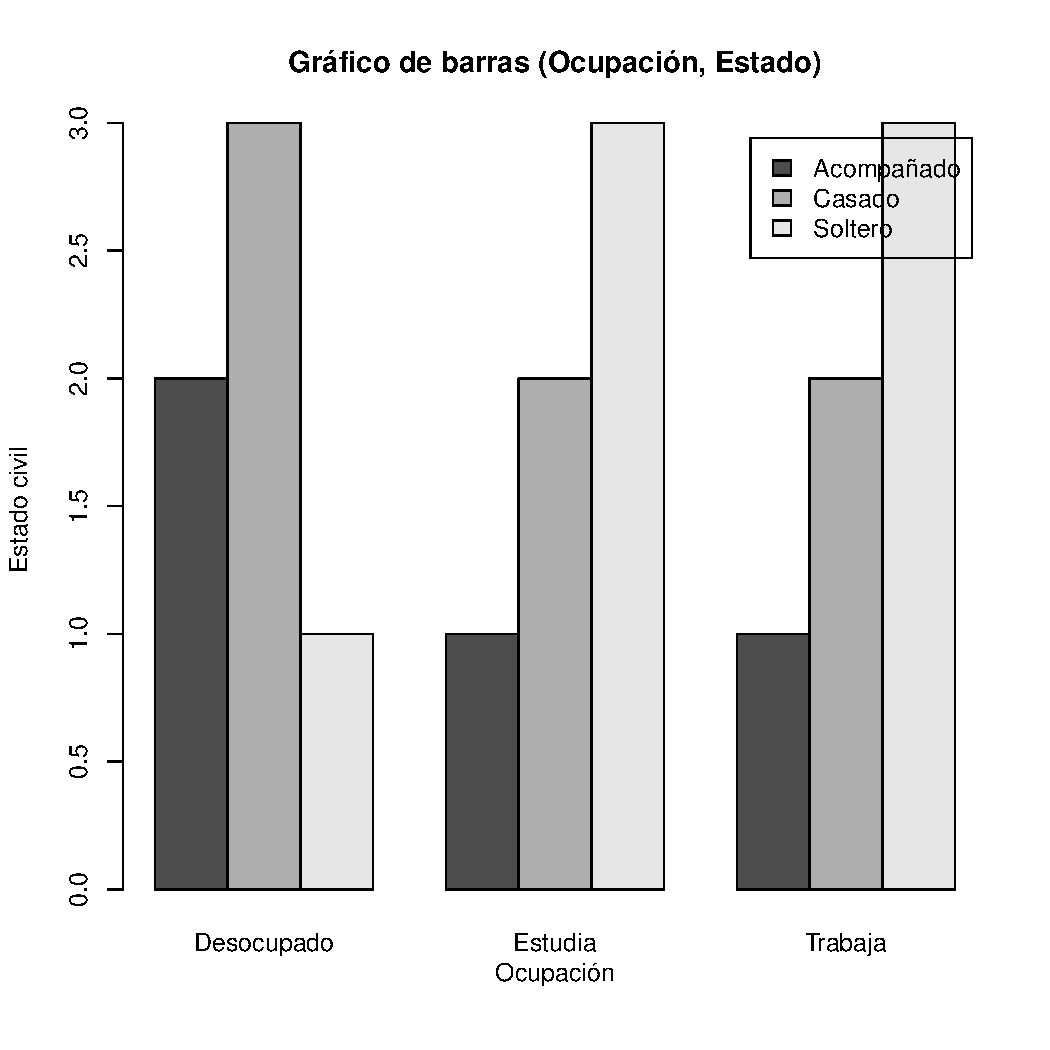
\includegraphics[width=\maxwidth]{figure/unnamed-chunk-1-3} 
\begin{kframe}\begin{alltt}
\hlkwd{plot}\hlstd{(}\hlkwd{ecdf}\hlstd{(x.norm),}\hlkwc{main}\hlstd{=}\hlstr{"Funci�n de distribuci�n acumulada te�rica"}\hlstd{)}
\end{alltt}
\end{kframe}
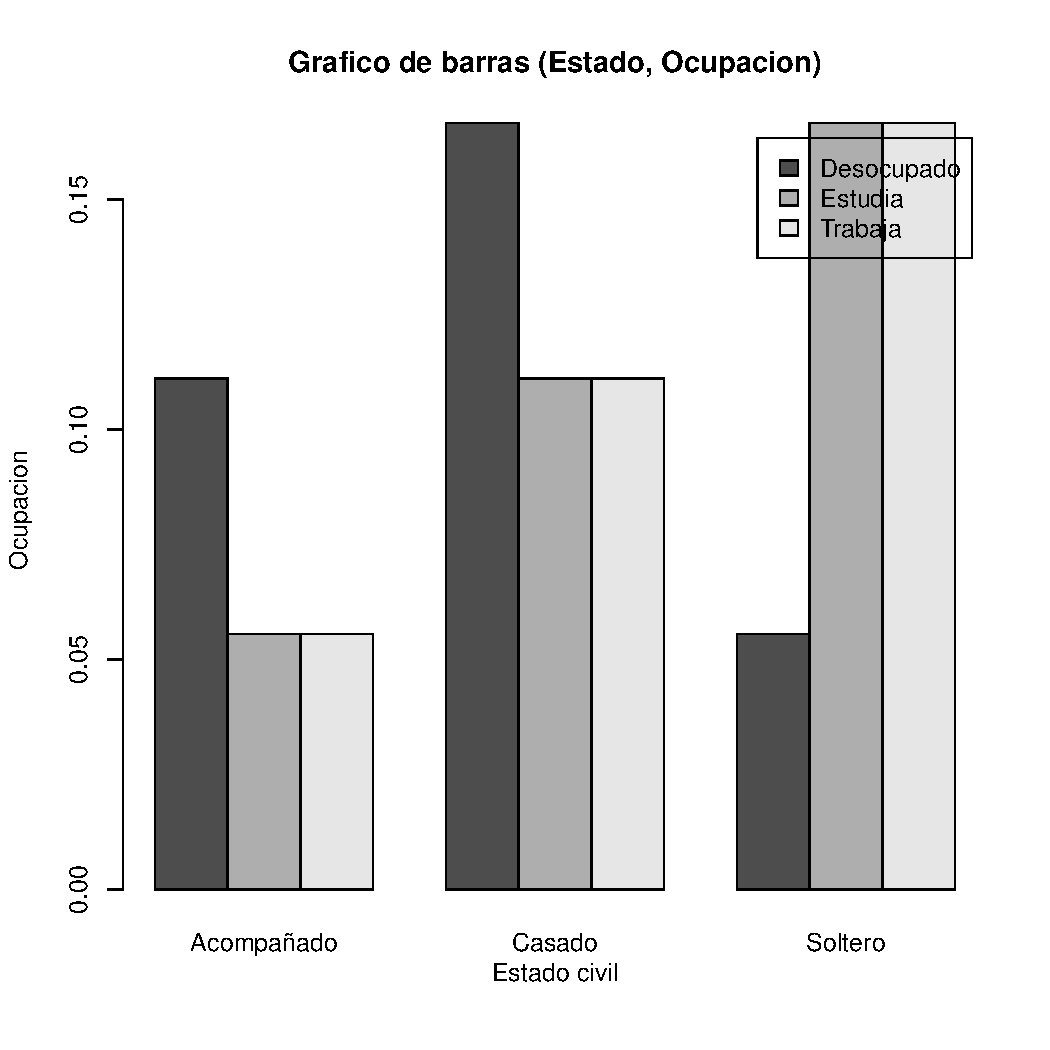
\includegraphics[width=\maxwidth]{figure/unnamed-chunk-1-4} 
\begin{kframe}\begin{alltt}
\hlcom{# Definir los par�metros apropiados}
\hlstd{media} \hlkwb{<-} \hlnum{4.5}\hlstd{; desviacion} \hlkwb{<-} \hlnum{0.75}
\hlcom{#Generar 100 n�meros aleatorios de la distribuci�n}
\hlstd{x} \hlkwb{=} \hlkwd{rnorm}\hlstd{(}\hlnum{100}\hlstd{, media, desviacion); x}
\end{alltt}
\begin{verbatim}
##   [1] 4.029920 5.821386 4.641438 3.449032 3.627814 3.935307 3.758119
##   [8] 5.915371 3.792341 3.529290 4.584295 4.024424 4.249860 4.009177
##  [15] 5.070156 4.204805 3.684109 2.772989 4.377355 5.917758 3.018638
##  [22] 4.568907 4.569531 6.004569 4.734568 3.371605 4.483181 4.290884
##  [29] 4.634000 3.555631 4.935092 6.247813 4.930580 4.712999 4.694150
##  [36] 4.535441 4.058150 5.181461 4.363378 4.548020 5.349070 4.423880
##  [43] 3.822976 3.297098 4.842226 4.455268 4.818021 5.270818 3.815976
##  [50] 4.108719 4.029195 4.141446 3.919951 3.609675 3.780259 5.338455
##  [57] 5.214300 4.233535 6.347621 3.723949 5.075039 3.744412 4.758563
##  [64] 3.894228 3.383547 3.886360 5.796572 4.351904 4.872332 4.528315
##  [71] 4.531842 4.927489 5.464806 5.025385 4.082680 3.297737 5.214124
##  [78] 4.084597 4.566551 4.445609 4.622740 4.576680 5.052774 3.797365
##  [85] 3.654596 5.209509 2.983339 5.280811 4.795568 4.900734 4.049733
##  [92] 4.624722 5.341009 4.282888 5.785911 3.736081 4.949583 4.593777
##  [99] 4.613655 4.797490
\end{verbatim}
\begin{alltt}
\hlcom{# Histograma para la nuestra aleatoria de tama�o 100}
\hlkwd{hist}\hlstd{(x,}\hlkwc{main}\hlstd{=}\hlkwd{expression}\hlstd{(}\hlkwd{paste}\hlstd{(}\hlstr{"X ~ N("}\hlstd{, mu,} \hlstr{" = 4.5, "}\hlstd{, sigma,} \hlstr{" = 0.75)"}\hlstd{)),} \hlkwc{xlab}\hlstd{=}\hlstr{"X"}\hlstd{,} \hlkwc{ylab}\hlstd{=}\hlstr{"densidad
de probabilidad"}\hlstd{,} \hlkwc{probability}\hlstd{=}\hlnum{TRUE}\hlstd{,} \hlkwc{col}\hlstd{=}\hlkwd{gray}\hlstd{(}\hlnum{0.9}\hlstd{))}
\hlkwd{curve}\hlstd{(}\hlkwd{dnorm}\hlstd{(x, media, desviacion),} \hlkwc{col}\hlstd{=}\hlstr{"red"}\hlstd{,} \hlkwc{lwd}\hlstd{=}\hlnum{2}\hlstd{,} \hlkwc{add}\hlstd{=}\hlnum{TRUE}\hlstd{)}
\end{alltt}
\end{kframe}
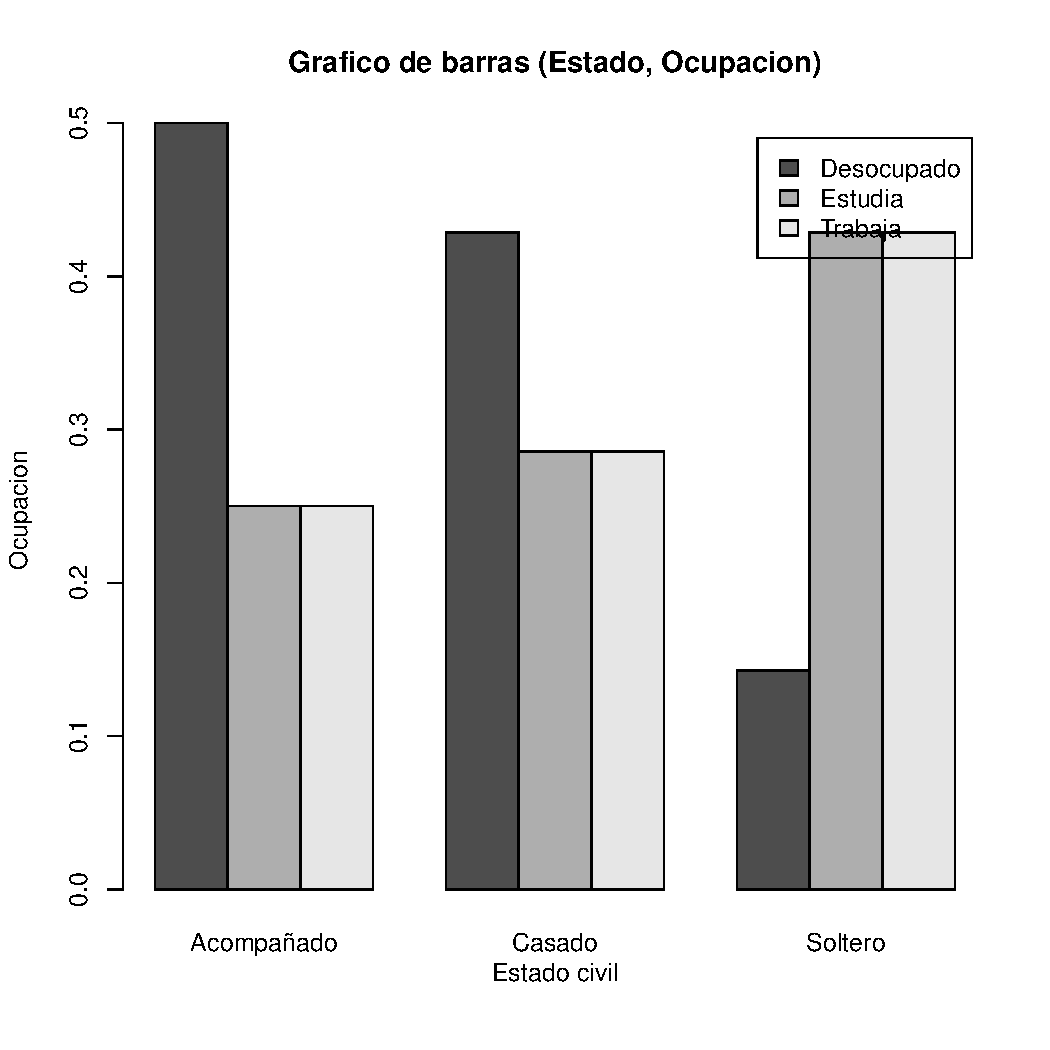
\includegraphics[width=\maxwidth]{figure/unnamed-chunk-1-5} 
\begin{kframe}\begin{alltt}
\hlcom{# Definir el par�metro apropiado}
\hlstd{media} \hlkwb{<-} \hlnum{2500}\hlstd{; razon} \hlkwb{<-} \hlnum{1}\hlopt{/}\hlstd{media;n}\hlkwb{=}\hlnum{100}
\hlcom{# generar 100 n�meros aleatorios de la distribuci�n}
\hlstd{x} \hlkwb{=} \hlkwd{rexp}\hlstd{(n, razon); x}
\end{alltt}
\begin{verbatim}
##   [1] 19760.35572   307.75717  5619.60345  2559.45081  4001.14564
##   [6]  1176.34429 13891.49632  1175.76155   389.79929  3242.60891
##  [11]   712.13648   862.90596  1895.92928  6033.00871  4178.98859
##  [16]  3213.49653  2831.33511  1862.33767  3790.25644   102.35523
##  [21]   572.85660  1362.69657    41.77218  1409.35913  2116.03617
##  [26]  2873.05052   909.01085  4016.74853   834.97153   897.77319
##  [31]  2764.45945   766.67769   926.10437    34.80731   864.51839
##  [36]  2185.20984   828.51697  1379.21548   697.26236   605.44715
##  [41]  1942.30793  1041.32961   137.68112  5635.62383  1017.62088
##  [46]  6117.64887  6605.00451  1823.57488  3268.44387  1161.68630
##  [51]  1325.85331   985.74760   971.46592  2570.25076   661.17817
##  [56]  1659.41369  1432.45270   401.57865  5781.98247  3077.51985
##  [61]   442.29178   257.39089  2178.98322   226.08883  2105.56829
##  [66]  2731.48244  1979.25972  4852.03465  3176.73497  3674.89756
##  [71]   901.98397  1117.61819  2445.20432  4029.85698  2136.55071
##  [76]  5719.89317  1194.77528  2232.32886  3677.43191   386.57073
##  [81]  1232.50977   902.41699   338.88838  1503.28907   803.62819
##  [86]  2195.38963   873.26272  3323.61484   152.24885  7138.52412
##  [91]   552.95901  3611.55573  1260.97157  1769.35024  3534.44546
##  [96]  1579.08208  2503.20230  3371.44982   269.78498  1037.28200
\end{verbatim}
\begin{alltt}
\hlcom{# Histograma para la nuestra aleatoria de tama�o 100}
\hlkwd{hist}\hlstd{(x,} \hlkwc{main}\hlstd{=}\hlstr{"X ~ Exponencial( media = 2500 )"}\hlstd{,} \hlkwc{xlab}\hlstd{=}\hlstr{"X"}\hlstd{,} \hlkwc{ylab}\hlstd{=}\hlstr{"densidad de probabilidad"}\hlstd{,}
\hlkwc{probability}\hlstd{=}\hlnum{TRUE}\hlstd{,} \hlkwc{col}\hlstd{=}\hlstr{"green"}\hlstd{)}
\hlkwd{curve}\hlstd{(}\hlkwd{dexp}\hlstd{(x, razon),} \hlkwc{col}\hlstd{=}\hlstr{"blue"}\hlstd{,} \hlkwc{lwd}\hlstd{=}\hlnum{2}\hlstd{,} \hlkwc{add}\hlstd{=}\hlnum{TRUE}\hlstd{)}
\end{alltt}
\end{kframe}
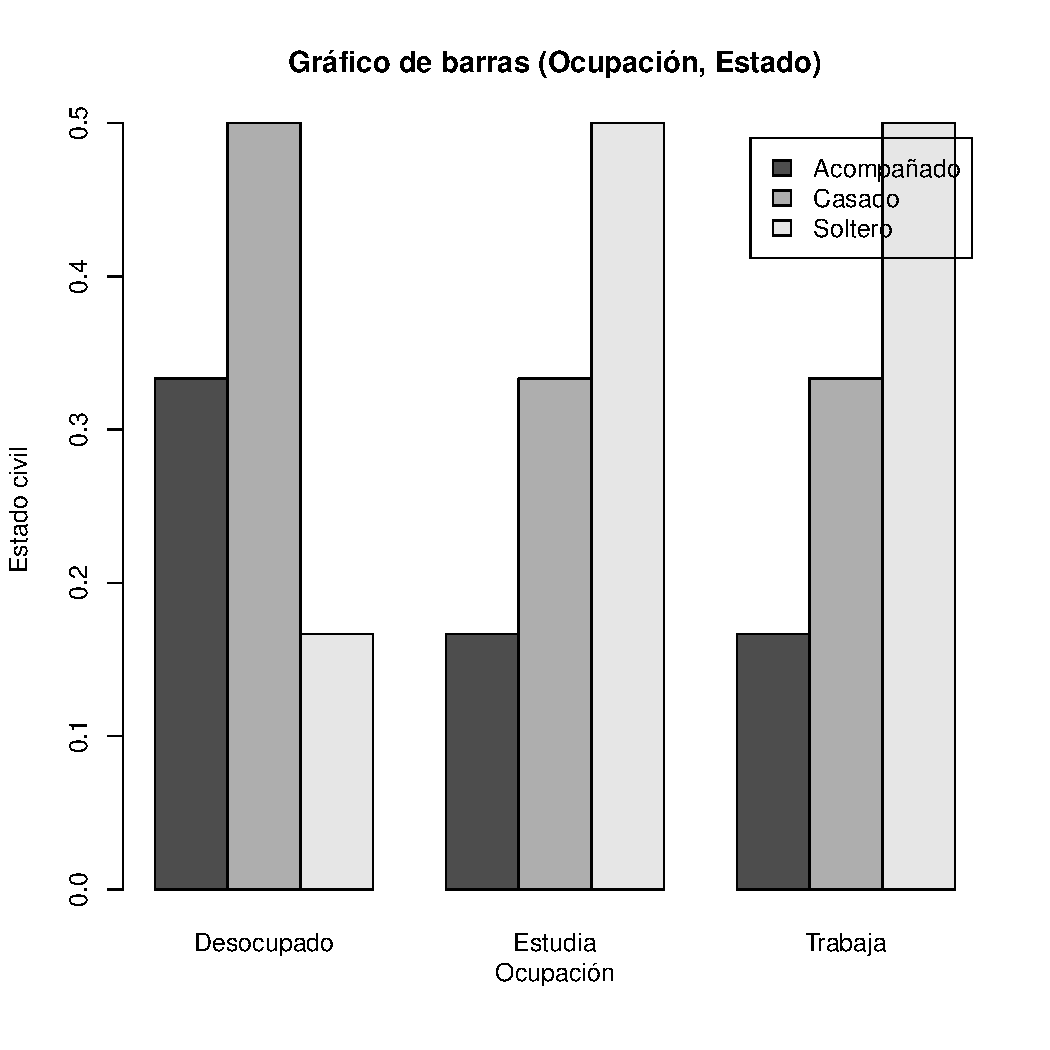
\includegraphics[width=\maxwidth]{figure/unnamed-chunk-1-6} 
\begin{kframe}\begin{alltt}
\hlstd{x} \hlkwb{<-} \hlnum{0.7}
\hlstd{p} \hlkwb{<-} \hlkwd{pnorm}\hlstd{(x,} \hlkwc{mean}\hlstd{=}\hlnum{1}\hlstd{,} \hlkwc{sd}\hlstd{=}\hlnum{1}\hlstd{,} \hlkwc{lower.tail} \hlstd{=} \hlnum{TRUE}\hlstd{); p}
\end{alltt}
\begin{verbatim}
## [1] 0.3820886
\end{verbatim}
\begin{alltt}
\hlstd{z} \hlkwb{<-} \hlnum{0.7}
\hlstd{p1} \hlkwb{<-} \hlkwd{pnorm}\hlstd{(z,} \hlkwc{mean}\hlstd{=}\hlnum{0}\hlstd{,} \hlkwc{sd}\hlstd{=}\hlnum{1}\hlstd{); p1}
\end{alltt}
\begin{verbatim}
## [1] 0.7580363
\end{verbatim}
\begin{alltt}
\hlstd{p2} \hlkwb{<-} \hlkwd{pnorm}\hlstd{(z,} \hlkwc{mean}\hlstd{=}\hlnum{0}\hlstd{,} \hlkwc{sd}\hlstd{=}\hlnum{1}\hlstd{,} \hlkwc{lower.tail}\hlstd{=}\hlnum{FALSE}\hlstd{); p2}
\end{alltt}
\begin{verbatim}
## [1] 0.2419637
\end{verbatim}
\begin{alltt}
\hlstd{p3} \hlkwb{<-} \hlnum{1}\hlopt{-}\hlkwd{pnorm}\hlstd{(z,} \hlkwc{mean}\hlstd{=}\hlnum{0}\hlstd{,} \hlkwc{sd}\hlstd{=}\hlnum{1}\hlstd{);p3}
\end{alltt}
\begin{verbatim}
## [1] 0.2419637
\end{verbatim}
\begin{alltt}
\hlstd{p} \hlkwb{<-} \hlnum{0.75}
\hlstd{z} \hlkwb{<-} \hlkwd{qnorm}\hlstd{(p,} \hlkwc{mean}\hlstd{=}\hlnum{0}\hlstd{,} \hlkwc{sd}\hlstd{=}\hlnum{1}\hlstd{,} \hlkwc{lower.tail} \hlstd{=} \hlnum{TRUE}\hlstd{); z}
\end{alltt}
\begin{verbatim}
## [1] 0.6744898
\end{verbatim}
\begin{alltt}
\hlstd{x} \hlkwb{<-} \hlnum{18.55}\hlstd{; gl} \hlkwb{<-} \hlnum{12}
\hlstd{p} \hlkwb{<-} \hlkwd{pchisq}\hlstd{(x, gl,} \hlkwc{lower.tail} \hlstd{=} \hlnum{FALSE}\hlstd{); p}
\end{alltt}
\begin{verbatim}
## [1] 0.09998251
\end{verbatim}
\end{kframe}
\end{knitrout}

\end{document}
